\documentclass{standalone}
\usepackage{tikz}
\usepackage{ctex,siunitx,ninecolors}
\setCJKmainfont{Noto Serif CJK SC}
\usepackage{tkz-euclide}
\usepackage{amsmath}
\usepackage{wasysym}
\usetikzlibrary{patterns, calc}
\usetikzlibrary{decorations.pathmorphing, decorations.pathreplacing, decorations.shapes,3d}
% \newcommand{\posthead}[2][gray]{
%   \begin{tikzpicture}[#2]
%     \fill[left color=#1,right color= #1,middle color=#1!20](0,0)ellipse(0.05 and 0.02);
%     \fill[left color=#1,right color= #1,middle color=#1!20](0.05,0)rectangle(-0.05,0.07);
%     \fill[left color=#1,right color= #1,middle color=#1!20](-0.06,0.07)arc(-180:0:0.06 and 0.02)--(0.06,0.15)--(0.05,0.16)--(-0.05,0.16)--(-0.06,0.15)--cycle;
%     \fill[#1!50!gray](0,0.16)ellipse(0.05 and 0.02);
%     \foreach \x in {75,45,15,-15,-45,-75}
%     {
%       \draw[very thin,#1!50!gray]({0.05*sin(\x)},{0.16-0.02*cos(\x)})--({0.06*sin(\x)},{0.15-0.02*cos(\x)})--++(0,-0.08);
%     }
%   \end{tikzpicture}
% }
\newcommand\dlj[2][0]{
  \begin{scope}[#2,scale=1.8]
    \begin{scope}[z={(10:10mm)},x={(150:10mm)}]
      \begin{scope}[canvas is yz plane at x=-0.25]
        \draw[fill=lightgray](0,-0.5)rectangle(-0.1,0.5);
      \end{scope}
      \begin{scope}[canvas is xy plane at z=-0.5]
        \draw[fill=darkgray](0.25,-0.1)rectangle(-0.25,0);
      \end{scope}
      \begin{scope}[canvas is zx plane at y=0]
        \draw[fill=gray](-0.5,-0.25)rectangle(0.5,0.25);
      \end{scope}
      \begin{scope}[canvas is yz plane at x=-0.2]
        \draw[fill=lightgray!50](0,-0.4)rectangle(1.2,0.4);
        \foreach \x in {-30,-20,...,20}
        {
          \draw[ultra thin] ([shift=(\x:0.6)]0.4,0)--++(\x:-0.1);
          \draw[ultra thin] ([shift=(\x+5:0.6)]0.4,0)--++(\x+5:-0.08);
          \foreach \y in {1,2,3,4,6,7,8,9}
          {
            \draw[ultra thin] ([shift=(\x+\y:0.6)]0.4,0)--++(\x+\y:-0.05);
          }
        }
        \draw[ultra thin] ([shift=(30:0.6)]0.4,0)--++(30:-0.1);
        \draw[very thin,red] (0.4,0)--++(#1:0.65)(0.4,0)--++(#1:-0.05);
        \draw[fill=gray](0.4,0)circle(0.02);
        \draw[very thin,fill=darkgray](0.3,-0.1)--++(0.15,0)arc(-90:90:0.1)--(0.3,0.1)--(0.3,0.05)--++(0.15,0)arc(90:-90:0.05)--(0.3,-0.05)--cycle;
        \draw[fill=cyan!20,fill opacity=0.5,very thin](0.3,-0.35)rectangle(1.1,0.35);
        \coordinate (in) at (0.2,0.25);
        \coordinate (out) at (0.2,-0.25);
        \fill[darkgray](in)circle(0.8pt)(out)circle(0.8pt);
      \end{scope}
      \begin{scope}[canvas is xy plane at z=-0.4]
        \draw[fill=darkgray](0.2,1.2)rectangle(-0.2,0);
      \end{scope}
      \begin{scope}[canvas is yz plane at x=-0.25]
        \draw[fill=lightgray!50](1.3,-0.45)rectangle(1.2,0.45);
      \end{scope}
      \begin{scope}[canvas is xy plane at z=-0.45]
        \draw[fill=darkgray](0.25,1.2)rectangle(-0.25,1.3);
      \end{scope}
      \begin{scope}[canvas is zx plane at y=1.3]
        \draw[fill=gray](-0.45,-0.25)rectangle(0.45,0.25);
      \end{scope}
    \end{scope}
    \node at (in)[below]{\scalebox{0.5}{$+$}};
    \node at (out)[below]{\scalebox{0.5}{$-$}};
  \end{scope}
}
\begin{document}
\small
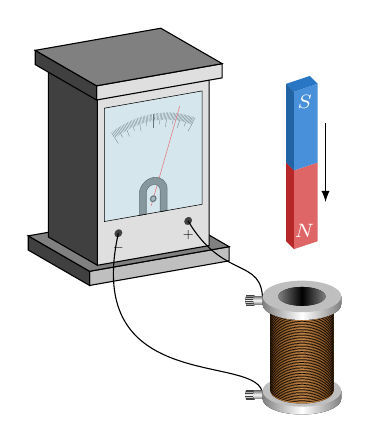
\begin{tikzpicture}[>=latex,scale=1.0]
  \dlj[17]{xshift=-2.2cm,yshift=2cm}
  \draw(in)..controls(-1.0,1.5)and(-0.5,1.8)..(-0.5,1.25);
  \draw(out)..controls(-2.8,0)and(-0.5,0.6)..(-0.5,0.05);
  \begin{scope}
    \foreach \y in {0.05,1.25}
      {
        \fill[top color=gray,bottom color=gray,middle color=white](-0.7,\y)ellipse(0.02 and 0.06);
        \fill[top color=gray,bottom color=gray,middle color=white](-0.7,\y-0.06)rectangle(-0.6,\y+0.06);
        \foreach \x in {75,45,15,-15,-45,-75}
        {
          \draw[very thin,darkgray]({-0.7-0.02*cos(\x)},{\y+0.06*sin(\x)})--++(0.1,0);
        }
        \fill[gray](-0.6,\y)ellipse(0.02 and 0.06);
        \fill[top color=gray,bottom color=gray,middle color=white](-0.6,\y)ellipse(0.02 and 0.05);
        \fill[top color=gray,bottom color=gray,middle color=white](-0.6,\y-0.05)rectangle(-0.5,\y+0.05);
      }
    \fill[left color=gray,right color=gray,middle color=white](-0.5,0)arc(-180:0:0.5 and 0.2)--(0.5,0.1)--(-0.5,0.1)--cycle;
    \fill[lightgray](0,0.1)ellipse(0.5 and 0.2);
    \fill[left color=brown4,right color=brown4,middle color=brown7](-0.4,0.1)arc(-180:0:0.4 and 0.16)--(0.4,1.2)--(-0.4,1.2)--cycle;
    \foreach \x in {0.12,0.14,...,1.18}
    {
      \draw[very thin](-0.4,\x)arc(-180:0:0.4 and 0.16);
    }
    \fill[lightgray](0,1.2)ellipse(0.4 and 0.16);
    \fill[left color=gray,right color=gray,middle color=white](-0.5,1.2)arc(-180:0:0.5 and 0.2)--(0.5,1.3)--(-0.5,1.3)--cycle;
    \fill[lightgray](0,1.3)ellipse(0.5 and 0.2);
    \fill[left color=gray,right color=gray,middle color=black](0,1.3)ellipse(0.3 and 0.12);
  \end{scope}
  \begin{scope}[yshift=2cm]
    \fill[red4](-0.2,0)--(-0.1,-0.1)--(-0.1,0.9)--(-0.2,1.0)--cycle;
    \fill[red6](-0.1,-0.1)--(0.2,0)node[inner sep=1pt,above left,text=white]{\scriptsize $N$}--(0.2,1.0)--(-0.1,0.9)--cycle;
    \fill[azure4](-0.2,1)--(-0.1,0.9)--(-0.1,1.9)--(-0.2,2.0)--cycle;
    \fill[azure6](-0.1,0.9)--(0.2,1)--(0.2,2.0)--(-0.1,1.9)node[inner sep=1pt,below right,text=white]{\scriptsize $S$}--cycle;
    \fill[azure5](-0.2,2)--(-0.1,1.9)--(0.2,2)--(0.1,2.1)--cycle;
    \draw[->](0.3,1.5)--++(0,-1);
  \end{scope}
\end{tikzpicture}
\end{document}